\documentclass[18pt,oneside,a4paper, titlepage]{article}

\usepackage[hidelinks]{hyperref}
\usepackage[pdftex]{graphicx}
\usepackage{amsmath}
\usepackage{algorithm}
\usepackage{algorithmicx}
\usepackage{algpseudocode}
\usepackage{lscape}
\usepackage{pdflscape}

\begin{document}
\begin{figure}[t]
	\centering
	
\includegraphics[scale=0.35]{logo-polimi.png}
\end{figure}
\title{\textbf{myTaxiService}\\\textbf{D}esign \textbf{D}ocument\\ A.Y. 2015/2016\\
	Politecnico di Milano \\ Version 1.0}	
\author{Cattaneo Michela Gaia, matr. 791685\\Barlocco Mattia, matr. 792735 }
\date{December 4, 2015}
\maketitle

\newpage
	\tableofcontents

\newpage
	%\documentclass[18pt,oneside,a4paper, titlepage]{article}	
	
%\begin{document}


\newpage
\section{Introduction}		
	\subsection{Purpose}
		This document represents the Design Document, which main goal is to describe the overall system architecture and to show the technical design decisions made, with the support of schema and diagrams.\\ It delineates how the software system will be structured in order to satisfy the requirements defined in the Requirement Analysis and Specification Document (RASD), each one translated into a representation of components, interfaces, and data necessary in the implementation phase.
		\\This document is addressed to the project development teams, technical architects, database designers and testers, as long as it has useful guidelines and a specific description of the design implementation of the system.
		
	\subsection{Scope}
		The system aims at simplifying the access of the passengers and guaranteeing a fair management of taxi queues.\\
		The server listens for the requests of the clients, which can be taxi drivers or users and access to their GPS position.\\
		The user clients are able to request a taxi and, if logged into the system, they can also make reservations and choose the payment method they prefer. On the other hand, taxi driver clients can change their status from available to unavailable, accept or decline the requests of the users and see their position in the queue of the area they are in.\\The server manages the notifications to forward to the clients, for example the arrival of a taxi for a user or the requests of the users for the taxi drivers. 
	
	\subsection{Definitions, Acronyms, Abbreviations}
		\begin{itemize}
			\item \textbf{Definitions}
				\item[-] \textbf{User}: a person who requests a service from the system. It can be a visitor or a passenger.
				\item[-] \textbf{Visitor}: a person who is not registered in the application.
				\item[-] \textbf{Passenger}: a person who is registered in the application.
				\item[-] \textbf{Taxi driver}: a taxi driver who access the application with a specific ID.
				\item[-] \textbf{Request}: the request of a taxi in a certain area and position in the city made by a user.
				\item[-] \textbf{Reservation}: the reservation of a taxi in a certain area, place and time that can be made only by passengers.
	\newpage
			\item \textbf{Acronyms and abbreviations}
				\item[-] \textbf{RASD}: Requirement Analysis and Specification Document
				\item[-] \textbf{DBMS}: Database Management System
				\item[-] \textbf{JEE}: Java Enterprise Edition
				\item[-] \textbf{API}: Application Programming Interface
				\item[-] \textbf{UML}: Unified Modeling Language
				\item[-] \textbf{HTML}: HyperText Markup Language
				\item[-] \textbf{HTTP}: HyperText Transfer Protocol
				\item[-] \textbf{MVC}: Model View Controller
			
		\end{itemize}
	\subsection{Reference documents}
		\begin{itemize}
			\item myTaxiService Requirement Analysis and Specification Document (RASD)
			\item  ISO/IEC/IEEE 42010:2011, Systems and software engineering — Architecture description
		\end{itemize}
	\subsection{Document structure}
		This document is divided in six main parts:
		\begin{itemize}
			\item \textbf{Introduction}: this section describes the document in general and its purpose.
			\item \textbf{Architectural Design}: this section specifies the architectural design part, giving information about the components involved.
			\item \textbf{Algorithm Design}: this section provides a general description of the main algorithms used during implementation.
			\item\textbf{ User Interface Design}: this section outlines an overview on how the user interfaces of the system will look like. 
			\item \textbf{Requirements Traceability}: this section explains the connection between the requirements already defined in the RASD and the design elements introduced in this document.
			\item \textbf{Appendix}: this section provides information about the tools used to redact this document and how many hours of work each author has spent. 
		\end{itemize}


%\end{document}
	%\documentclass[18pt,oneside,a4paper, titlepage]{article}

%\usepackage[hidelinks]{hyperref}
%\usepackage[pdftex]{graphicx}
%\usepackage{lscape}
%\usepackage{pdflscape}

%\begin{document}

\newpage
	\section{Architectural Design}
		\subsection{Overview}
			This section deals with the specific description of the architectural choices made for the myTaxiService system. These decisions are supported by different diagrams, whose aim is to highlight and simplify the view of the components of the system, and explanations about the architectural styles adopted.
			\\In the first subsections there is a representation of the components of the system with diagrams. Here are presented the high level components and their interaction, with a brief definition of the functionalities of the three components individuated, then these are unfolded and there is a more specific description of the components, the interfaces and their relationships and features.\\
			The last subsection explains and justifies the architectural styles selected for the myTaxiService system, which consists in a client/server, event-based system, with a service-oriented, three tier architecture (client, server and database). 
			
	
\newpage
		\subsection{High level components and their interaction}
		% here you can introduce the high level components of your architecture (in our basic example in the slides about design you find these in slide 7) and describe the main interaction between them (no details here. You can say why some components talk to each other, why, if the communication is synchronous or asynchronous, any other info you think is useful at this point). 
			\vspace{1cm}
			\begin{figure}[h]
				\centering
				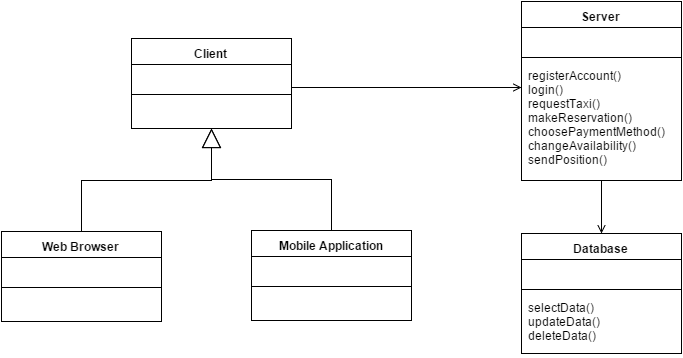
\includegraphics[scale=0.45]{Diagrams/HighLevelComp2.png}
			\end{figure}
			\vspace{1cm}
			\begin{itemize}
				\item \textbf{Client}: this part runs on the client devices via a Web browser or the mobile application. It allows the users to insert and submit the data in the input forms, that are sent to the application server. On the other hand, the taxi drivers can send information about their availability to the server and the application client monitors their GPS position in order to move the taxi drivers to another queue if they change their area. 
				\item \textbf{Application Server}: this part runs on the JEE server. It is composed of a web server part, which always listens to all the clients requests and is responsible for the creation of the faces and pages of the client interfaces. The application server, instead, contains the logical part of the application, collecting and managing the information from the clients and the database. In fact, it analyses the data coming from the clients and, according to the requests, it modifies or asks for the required information stored in the database, then it is able to answer the client request, sending it the result.  
				\item \textbf{Database}: this part contains the database where all the application data are stored. It is not only accessed by the application server, but also by the administrators, who can, for example, directly add a taxi driver account to the database. 
			\end{itemize}	
			
	\newpage
		\subsection{Component view}
		% here you have a refinement of what you have in Section 4.B and identify sub-components. For instance, the diagram in slide 6 could be a diagram showing a  component view
		These are the components that define the myTaxiService system architecture. This diagram is composed by many subsystems and an external component which belongs to the database.\\ Starting from the left, in the first subsystem, the \textbf{Controller}, there are two components that manage the requests of the users and the payments.\\ The \textit{RequestManager} component manages all the logic of the requests, getting the information from the users and forwarding them to the designated taxi driver. As it deals with several tasks, he needs more than one interface to be implemented: \textit{RequestTaxiVisitor}, \textit{Notifications}, \textit{RequestTaxiPassenger} and \textit{MakeReservation} are the required interfaces for this component. It also relates with other components: it uses the \textit{PaymentManager} and the \textit{Data}, in order to complete its operations, and creates the \textit{ChoosePaymentMethod} interface, which is required by the \textit{PaymentManager}.\\
		The second subsystem is called \textbf{Functions}, as it provides the possible actions that the user can do while using the system. It is composed by four interfaces provided to the \textbf{Controller}: \textit{PaymentManager}, \textit{RequestTaxiPassenger}, \textit{MakeReservation} and \textit{Notifications}.\\
		This last interface can be accessed from the taxi driver mobile application to see the notifications of the requests, in fact it is produced by the \textit{TaxiDriverArea} interface.
		The \textit{RequestTaxiPassenger} and \textit{MakeReservation} interfaces, instead, are created by the \textit{PassengerArea} interface, which is part of the subsystem \textbf{Account} with \textit{TaxiDriverArea}. They are used by the passenger when he needs to request a taxi or make a reservation from his personal area.\\
		Another subsystem is the \textbf{AccountManager} whose main goal is to manage the access of the users, forwarding them to the proper designated area. The \textit{TaxiDriverAreaManager} requires the interface \textit{TaxiDriverArea}, which is provided by the \textit{TaxiDriverArea} interface in \textbf{Account}. The same relation is defined between the \textit{PassengerAreaManager} component and the \textit{PassengerArea}. The third component of this subsystem, the \textit{AccessManager}, which is responsible for the log in and the registration of the users, creates an instance of \textit{PassengerArea}, while requires the interface \textit{Access}.\\
		The last subsystem is the \textbf{Visitor}, which provides the interface \textit{Access} to the \textit{AccessManager} and another interface, \textit{RequestTaxi} to the \textit{RequestManager}. In fact, this subsystem represent the home page where the visitor can register or log in and request a taxi.
		
		
		\begin{landscape}
			\newpage
			\begin{figure}[!h]
				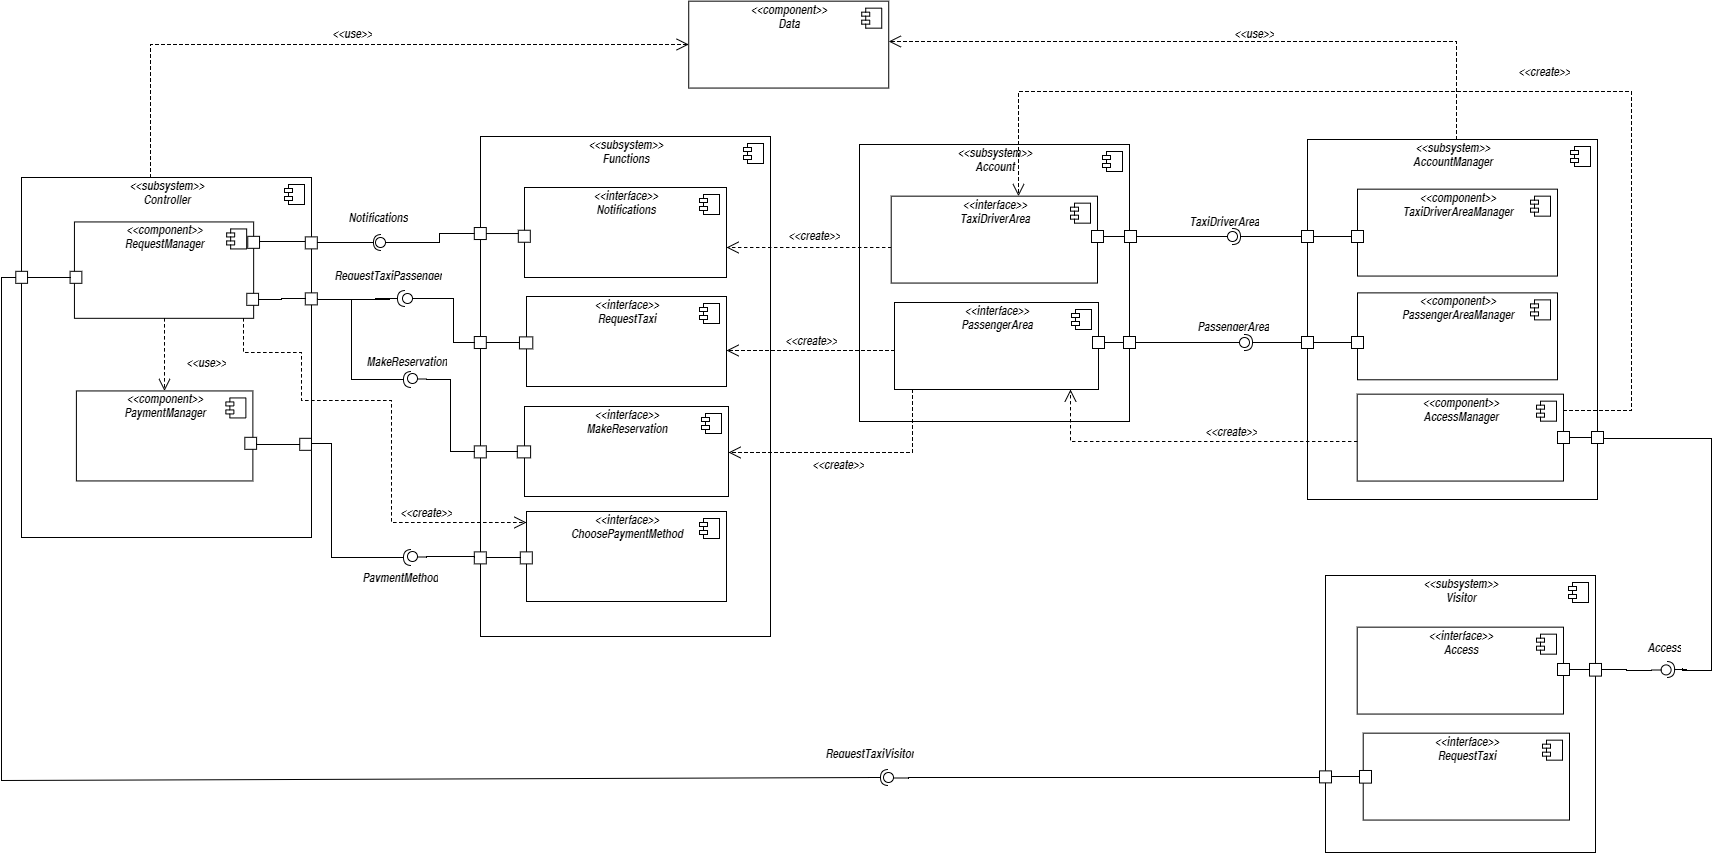
\includegraphics[scale=0.41]{Diagrams/componentDiagram.png}
			\end{figure}
		\end{landscape}
		
	\newpage	
		\subsection{Deployment view}
		% this is what you have in slide 8, that is, the identification of the artifact that need to be deployed to have the system working
		\vspace{0,7cm}
		\begin{figure}[h]
			\centering
			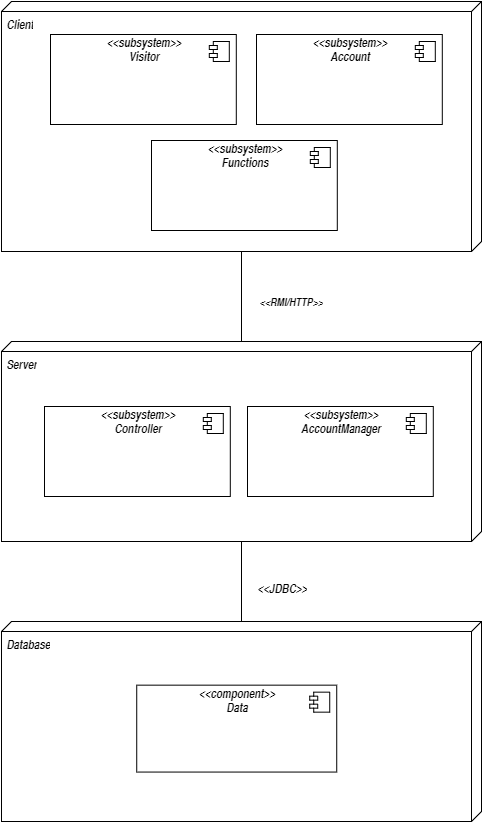
\includegraphics[scale=0.56]{Diagrams/deploymentDiagram.png}
		\end{figure}
	\newpage
		\subsection{Runtime view}
		%	You can use sequence diagrams to describe the way components interact to accomplish specific tasks typically related to your use cases
		% this is what you have in slide 9 plus sequence diagrams describing the way components behave in order to accomplish a certain activity
		\vspace{2cm}
			\begin{figure}[h]
				\centering
				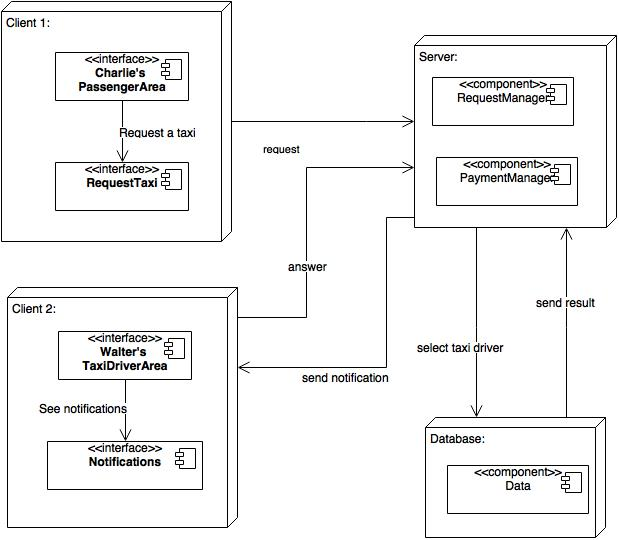
\includegraphics[scale=0.65]{Diagrams/runTime.jpg}
			\end{figure}
		%other sequence
	\newpage
		\subsection{Component interfaces}
		% here you define the interfaces of your components, that is, which operations they offer to the external world, their meaning, any input and output parameter (name, possible set of values/type)
		Here is presented a list of the interfaces defined in the component diagram and their functionalities.
		\begin{itemize}
			\item \textbf{Access.}
			\item \textbf{TaxiDriverArea.}
			\item \textbf{PassengerArea.}
			\item \textbf{RequestTaxiVisitor.}
			\item \textbf{RequestTaxiPassenger.}
			\item \textbf{MakeReservation.}
			\item \textbf{PaymentMethod.}
		\end{itemize}
	\newpage
		\subsection{Selected architectural styles and patterns}
		%	Please explain which style/patterns you used, why and how
		\begin{itemize}
			\item \textbf{Client/Server.} The client/server architecture is the optimal solution for the myTaxiService system, as it is necessary to have a central system that listens, manages and forwards the requests of the different clients. There is a central server that contains the logic of the application and the clients are the users of the system, such as visitors, passengers and taxi drivers.
			\item \textbf{Three-tier.} It has been adopted a three-tier architectural model, composed by thin client, application server and database.\\ This architecture is the best choice for our system, even if it has some cons, such as the complexity of the structure and the difficulty of set up and maintenance, it still has several pros. For example, it guarantees increased performance and great flexibility, useful if there will be any future change concerning the architecture. Moreover it is granted a great security level, thanks to the decoupling of logic, data and presentation, which is essential as the system deals with several personal data.
			\item \textbf{Event-Based System.} The myTaxiService application is based on the event firing. \\It is necessary, in fact, that the system is reactive and that does different quick operations according to the action of the clients. For example the visitors and passengers make requests and reservations, which the system has to manage and forward to the first taxi of the area, and the taxi drivers can change their availability state and the system has to start or end the monitoring of their position, and they can accept or decline a request and the system has to manage the queue. \\The users and the taxi drivers are registered to different events and expect to receive notifications about what they need, whether it is the arrival of a taxi or the requests of the users.\\ The events are asynchronous and based on a "send and forget" paradigm, where the system only cares for sending the notifications to the designated clients or doing the actions needed in response of the event fired.
			\item  \textbf{Service-Oriented Architecture.} A service-oriented architecture is necessary if the system wants to be more flexible and expandable. In fact, the myTaxiService application needs to provide programmatic interfaces in order to be open to future implementations of additional services. This can be guaranteed with this architectural choice, which is based on the loose coupling of the services, allowing to easily add more functionalities, without starting from scratch when a change is needed, and to simplify the maintenance of the system.
		\end{itemize}
							
%\end{document}	
	\documentclass[18pt,oneside,a4paper, titlepage]{article}
\begin{document}
	
	\newpage
	
	\section{Algorithm Design}
	%	Focus on the definition of the most relevant algorithmic part of your project
		The most relevant algorithm of the myTaxiService application is the one implementing the queue management. It is important to optimize its implementation as long as it is the most complex and the one that distinguishes the system.\\
		\begin{itemize}
			\item INIT: There is a class that initializes the queues of the taxi drivers, starting assigning one taxi to all the areas and then, basing on the statistics data, the queues are filled with a number of taxi drivers that is greater or equal than the number of the requests expected in that area.\\
			COMPLEXITY: O(T) with T=number of taxis (randomly assigned)
			\item REQUEST: The taxi drivers are now able to take requests in the designated area. When a taxi driver takes a request the system sets his availability to false and it stops monitoring his position. In fact, the server constantly monitors the position of all the taxi drivers that are declared available, connecting to the GPS on their devices, and uses this values in order to manage the taxi distribution in the different areas. If a taxi driver does not accept the request of a user, whether because he is busy or because he has not seen the call in the first minute, the system moves him to the last position of the queue, forwarding the request to the second one.\\
			COMPLEXITY: O(A+Q) with A=number of areas and Q=number of taxi in queue in that area(find the area where the passenger is in and take the first of the queue of that area)
			\item QUEUES: The areas of the city are represented by a graph with an array of adjacencies and the queue of the taxi drivers, whose position is within its boundaries, is assigned to each area. It is a useful representation in order to decide how to distribute the taxis, in fact it is possible that an area is occupied by a number of taxi that is equal to the threshold of the maximum taxis that can be present in that area. In this case the system does not put a recently arrived taxi in the queue of that area, but advise the taxi driver that he will be moved to an adjacent area that has the minimum number of taxi, searching recursively in the adjacencies of the areas. As it is necessary to guarantee that there should always be at least one taxi driver in each area, when it occurs that the last taxi driver leaves an area, the system instantly notifies the last taxi driver of the queue that he has to move from the most populated adjacent area to the needy area.
			COMPLEXITY: O(A)
		\end{itemize}
		
		%the complexity of the algorithms
	ADD DOMAIN PROPERTY: ALMENO UN TAXI ACCETTA LA RICHIESTA.
	
	
\end{document}
\newpage	
	\section{User Interface Design}
		The user interface design has been already specified in the section 3.1.1 of the RASD, where all the user interfaces are described with the support of mockups.
	%	Provide an overview on how the user interfaces of your system will look like. If you have already included this part in the RASD you can simply refer to what you have already done, possibly providing here some extensions if applicable.
		In order to show in a simplified way the steps through the different screens, it has been used the UX diagram, one to illustrate the user interfaces and the other for the taxi driver ones.
		\subsection{Taxi driver UX diagram}
		\vspace{1cm}
		\begin{figure}[h]
			\centering
			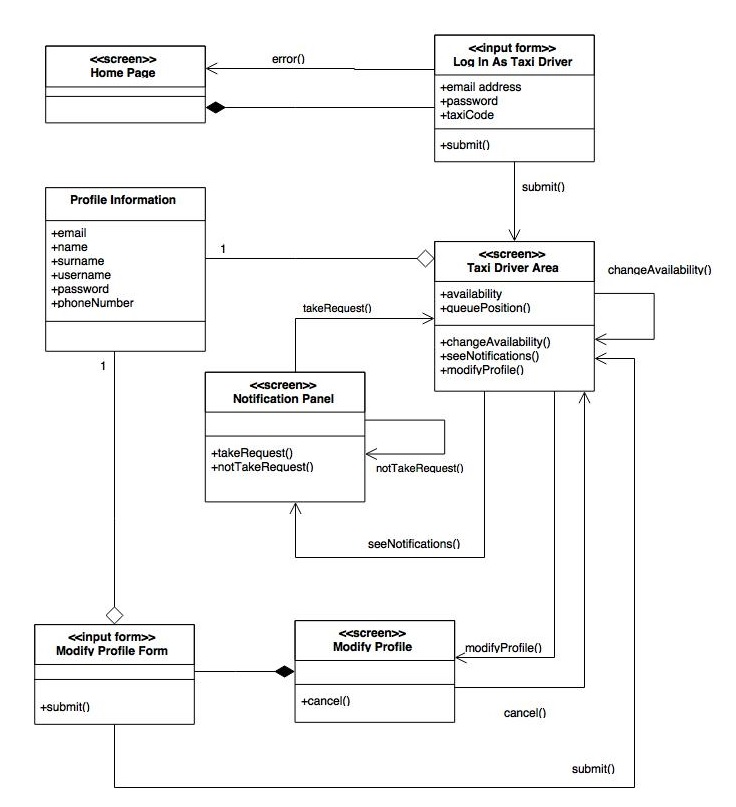
\includegraphics[scale=0.7]{Diagrams/UXDiagramTaxiDriver.jpg}
		\end{figure}
		
		\newpage
		\subsection{User UX diagram}
			\vspace{1.5cm}
		\begin{figure}[h]
			\centering
			\includegraphics[scale=0.46]{Diagrams/UXDiagramPassenger.jpg}
		\end{figure}
\newpage
	\section{Requirements Traceability}
	%	Explain how the requirements you have defined in the RASD map into the design elements that you have defined in this document.
		\begin{itemize}
			\item \textbf{Registration of the visitor.} This requirement is specified in section 2.3 in the "Access" interface and in the "AccessManager" component.\\ It is also defined in section 4 in the "Sign Up" screen and in the "Sign Up Form" input form.
			
			\item \textbf{E-mail confirmation.} This requirement is specified in section 4 in the "Sign Up Form" input form.
			
			\item \textbf{Look up information about the system.} This requirement is specified in section 4 in the "Home Page" screen.
			
			\item \textbf{Log in as a passenger.} This requirement is specified in section 2.3 in the "Access" interface and in the "AccessManager" component.\\ It is also defined in section 4 in the "Log In As Passenger" input form.
		
			\item \textbf{Log in as a taxi driver.} This requirement is specified in section 2.3 in the "AccessManager" component.\\ It is also defined in section 4 in the "Log In As Taxi Driver" input form.
		
			\item \textbf{Log in with social networks.} This requirement is specified in section 2.3 in the "Access" interface and in the "AccessManager" component.\\ It is also defined in section 4 in the "Log In As Passenger" input form.
			
			\item \textbf{Retrieve password.} This requirement is specified in section 2.3 in the "AccessManager" component.
			
			\item \textbf{Request a taxi.} This requirement is specified in section 2.3 in the "RequestTaxi" interface and in the "RequestManager" component.\\ It is also defined in section 4 in the "Passenger Area" screen.
			
			\item \textbf{Reserve a taxi.} This requirement is specified in  section 2.3 in the "MakeReservation" interface and in the "RequestManager" component.\\ It is also defined in section 4 in the "Reservation" screen and "Reservation Data" input form.
			
			\item \textbf{Choose payment method.} This requirement is specified in section 2.3 in the "ChoosePaymentMethod" interface and in the "PaymentManager" component.\\ It is also defined in section 4 in the "Choose Payment Method" screen.
			
			\item \textbf{View profile.} This requirement is specified in section 2.3 in the "PassengerArea" and "TaxiDriverArea" interfaces.\\ It is also defined in section 4 in the "Passenger Area" screen.
			
			\item \textbf{Edit profile.} This requirement is specified in section 2.3 in the "PassengerArea" and "TaxiDriverArea" interfaces and in the "PassengerAreaManager" and "TaxiDriverAreaManager" components.\\ It is also defined in section 4 in the "Modify Profile" screen and "Modify Profile Form" input form.
			
			\item \textbf{See waiting time.} This requirement is specified in section 4 in the "Waiting For A Taxi" screen.
			
			\item \textbf{Change availability.} This requirement is specified in section 2.3 in the "TaxiDriverArea" interface and in the "TaxiDriverAreaManager" component. \\ It is also defined in section 4 in the "Taxi Driver Area" screen.
			
			\item \textbf{Notification of the requests.} This requirement is specified in section 2.3 in the "TaxiDriverArea" interface and in the "TaxiDriverAreaManager" component. \\ It is also defined in section 4 in the "Notification Panel" screen.
			
			\item \textbf{See position in the queue.} This requirement is specified in section 2.3 in the "TaxiDriverArea" interface and in the "TaxiDriverAreaManager" component. \\It is also defined in section 4 in the "Taxi Driver Area" screen.
		\end{itemize}

	\section{References}
		\begin{itemize}
			\item  ISO/IEC/IEEE 42010:2011, Systems and software engineering - Architecture description
			\item UML Component Diagrams\\ (\url{http://www.uml-diagrams.org/component-diagrams.html})
			\item Introduction to the Diagrams of UML 2.X \\(\url{http://www.agilemodeling.com/essays/umlDiagrams.htm})
		\end{itemize}
\newpage
	\section{Appendix}
		\subsection{Software and tools used}
				\begin{itemize}
					\item TeXstudio (\url{http://www.texstudio.org/}): to redact and to format this document.
					\item draw.io (\url{https://www.draw.io/}): to create all the diagrams.
				\end{itemize}
		\subsection{Hours of work}
			Time spent redacting this document:
			\begin{itemize}
				\item Cattaneo Michela Gaia: {\raise.17ex\hbox{$\scriptstyle\sim$}}35 hours of work.
				\item Barlocco Mattia: {\raise.17ex\hbox{$\scriptstyle\sim$}}35 hours of work.
			\end{itemize}
		
		
		
\end{document}